\documentclass[12pt]{wlscirep}
\usepackage[utf8]{inputenc}
\usepackage{pst-all}
\usepackage{hyperref}
\usepackage[hidelinks]{hyperref}
\usepackage{float}
\usepackage{subcaption}

\setlength{\belowcaptionskip}{-0.2cm}
\title{Bayesian Statistical Analysis in PacMan}
\let\iif\leftrightarrow
\author[1]{Juan S. C\'ardenas Rodr\'iguez}
\author[2]{David Plazas Escudero}
\affil[1]{Universidad EAFIT, jscardenar@eafit.edu.co, Student, Medell\'in, Colombia}
\affil[2]{Universidad EAFIT, dplazas@eafit.edu.co, Student, Medell\'in, Colombia}
\usepackage{multicol}

\keywords{Bayesian Analysis, empirical distributions, PacMan.}

 \begin{abstract}
	On this paper, we use Bayesian inference and Markov chains to make the ghosts in the famous PacMan game to have more difficulty. This was done by calculating the probability of the most likely node that the player is going to be and, in this manner, making the ghost go to that node instead of following the player as the game does. It was achieved to code this algorithm and, it was proven that this probabilistic method did made more difficult the game, making people lose 10 seconds earlier (on average) than before. Therefore, we found that this types of method could be really useful for games with most complexity due to the fact that this allowed better ways to teach behavior to a character and, to add better ways to predict to make it more challenging to the gamer.
 \end{abstract}
\begin{document}

\flushbottom
\maketitle

\thispagestyle{empty}

\section{Introduction}
In the 1920s, Charles Ponzi duped investors when he convinced them that he will return a 50\% revenue every 90 days; he was actually paying the old investors with the money given by the new ones. This is known as the Ponzi Scheme nowadays; since the virtual currencies lack of regulation and have enhanced privacy for trading, they can be and are being used by fraudsters to perpetrate their frauds in similar fashion \cite{ponzi}.

\noindent In 2017, the cryptocurrency company BitConnect launched its new coin BitConnect Coin (BCC, not to be confused with BitCoin Cash), which assured every user that whatever investment they made in their currency and made part of their loan and exchange platform (which allowed them to loan the company USD and Bitcoin to the company in favor of some interests) they will return up to 40\% of their initial investment every month. After using broad marketing strategies to avoid their investors to know about their fraudulent intentions and recollecting thousands of investments, they closed the loan and exchange platform; so, all the people who invested in the BCC lost all their money because of the 96\% drop in the price of the coin. Even the company promised to return some money for the people who got affected by given them the average of the price of the coin in the last 15 days but, given that BCC was at such a low price there were several financial lossess by the investors. In this day and age, there are new companies like XRPConnect, EthConnect, Bunny Token and NEOConnect that are replicating the schemes that BCC made without any type of regulation which, as what happened with BitConnect, can lead to disastrous results \cite{nextWeb}.

\noindent In this manner, cryptocurrencies can over-inflate their price by artificially manipulating the price by marketing it with unrealistic expectations so people start buying the coin and in some delay, selling it to other people to obtain profit through the Exchanges or the Peer to Peer system, who would put more coins in the market through mining. As they exploit the price and people invest more in the coin, they then can abuse this by incrementing by a big margin their Exchange rate or, on the other side, the company changes the coins it possesses for USD or another currency and, proceed to devaluate their coin so they do not have to pay people back. \cite{bcc11}.

\noindent On the other hand, price leveraging is not as hard in cryptocurrencies as other stocks that are available in the market. An article written in the Journal of Monetary Economics about the price manipulation in the bitcoin system, that the sudden spike in the price of bitcoin in 2013 happened due to suspicious activity in an exchanges called ``Mt.Gox Bitcoin Currency Exchange'', which 600000 BTC valued at 188 million USD were acquiered using bots, artificially inflating the price without any real substance; the article explains how this could have a massive effect in the growth rate of BTC in a positive manner, reaching a 4\% growth rate each day after \cite{PMitBE}.

\subsection{Problem of cryptocurrencies}
Taking account of all the above, the cryptocurrency system allows for people to abuse it in fraudulent ways to augment the growth rate of the price of that coin without any type of repercusion, due to the lack of goverment regulation. On the other hand, as an articles of forbes says, most of investors in this currencies like this investment because of the same lack of government involvement \cite{forbes}. In this manner, nowadays companies like Bunny Token, ETH Connect, XRPConnect and mire are expecting 1\% growth in their price daily without any type of proof or security for the investors without too much control because, of the lack of control they have, leading to a easier atmosphere to scam people.

\indent To conclude, it's important to notice that even if the problem and the variables have a very short span, there can be found a lot of documentation about them because they were one of the trending topics last year. Most people see Bitcoin and other cryptocurrencies as a safe economic investment and a way to make easy profit. Although we are not saying that is something that we should thrive to eliminate completely, it is important to examine how this system works and start to make policies that makes investing in this opportunity a safer place for the consumer and, stop catastrophes like BitConnect to don't ever happen again.



\section{Theory \& Background}
\label{sec:theory}
	\subsection{Joint Distribution}\label{subsec:joint}
		In order to explain the model that will be presented, the notion of joint distribution needs to be introduced. Let's suppose we have a random vector $(X,Y)$, we can define a joint distribution as a function $F(x,y):\mathbb{R}^2\rightarrow[0,1]$ such that
        \begin{equation}
        	F(x,y)=P(X\leq x\,\,\wedge\,\, Y \leq y)
        \end{equation}
    	This is due to the fact that, just as a random variable, a random vector creates a probability measure, in this case, in $\mathbb{R}^2$; though, this can be perfectly scaled to a vector with $n$ random variables, inducing a probability measure in $\mathbb{R}^n$ \cite{rinconProb}.

        Following the theory from random variables, a random vector is completely defined with its joint distribution. A joint density function can also be defined over a random vector, even though, it may not exits. This is
        \begin{equation}
        	f(x,y)=P(X=x\,\,\wedge\,\,Y=y)
        \end{equation}

         In order to introduce the concept of independent random variables, we need to present the definition of marginal distribution. Let $(X,Y)$ a random vector with joint distribution $f(x,y)$, we define the joint distribution of X and Y, respectively (depending of the type of random vectors)
         \begin{align}
         	f_X(x)&=\sum_{y}f(x,y)\\
            &=\int_{-\infty}^\infty f(x,y)dy\\
            f_Y(y)&=\sum_xf(x,y)\\
            &=\int_{-\infty}^\infty f(x,y)dx
         \end{align}

         With these, we get the important result for independent random variables:
         \begin{equation*}
         	f(x,y)=f_X(x)f_Y(y) \quad \iif \quad \text{X,\,Y are independent}
         \end{equation*}

  \subsection{Finite state machines} \label{subsec:finite}
      A finite state machine is a computational model that is often used to simulate sequential logic and other computer programs. Finite state machines can be used to model problems in many fields including mathematics, artificial intelligence, games, and linguistics. They are completely described by a five-element tuple:
      \begin{multicols}{2}
      \begin{equation*}
      	(Q,\Sigma,\delta,q_0,F)
      \end{equation*}
      \columnbreak
      \begin{itemize}
      \item $Q=$ a finite set of states
      \item $\Sigma=$ a finite, nonempty input alphabet
      \item $\delta=$ a series of transition functions
      \item $q_0=$ the initial state
      \item $F=$ the set of accepting states
      \end{itemize}\end{multicols}

There are two types of finite state machines: deterministic and nondeterministic finite state machines. Both of them can be represented with the tuple, but the nondeterministic finite state machines do not have to have a transition function for every symbol in $\Sigma$, there can be multiple transition functions between states, and there can be null transitions, often represented with $\epsilon$, and they allow the machine to jump from one state to another without having to read a symbol \cite{brilliantFinite}.

    Figure \ref{img:finite} shows a deterministic finite machine diagram that describes a few simple moves that a character in a video game can do: stand, run, and jump. The buttons that a player can use to control this particular character are ``Up'', ``A'', or the player can press no button.
      \begin{figure}[H]
          \centering
          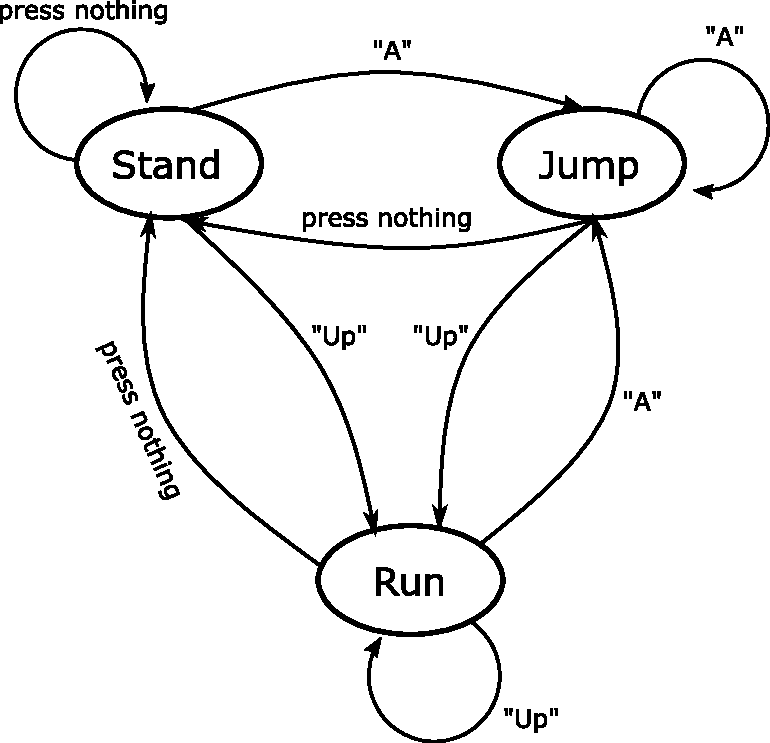
\includegraphics[scale=0.5]{files/Finite.pdf}
          \caption{Finite state machine for a video game character controlled by the player  \cite{brilliantFinite}.}
          \label{img:finite}
      \end{figure}

	\subsection{Markov Chains}
	A Markov Chain is a mathematical representation of a system that can pass from one state to another according to some defined probabilities to this transitions. The main characteristic of a Markov Chain is that the possible future states are independent from the initial state of the process. The set of possible states can be anything, depending on the problem at hand; for example, the states set can be letters, numbers, actions, etc. Figure \ref{img:markov} shows an example of a four-state chain for numbers.
    \begin{figure}[H]
        \centering
        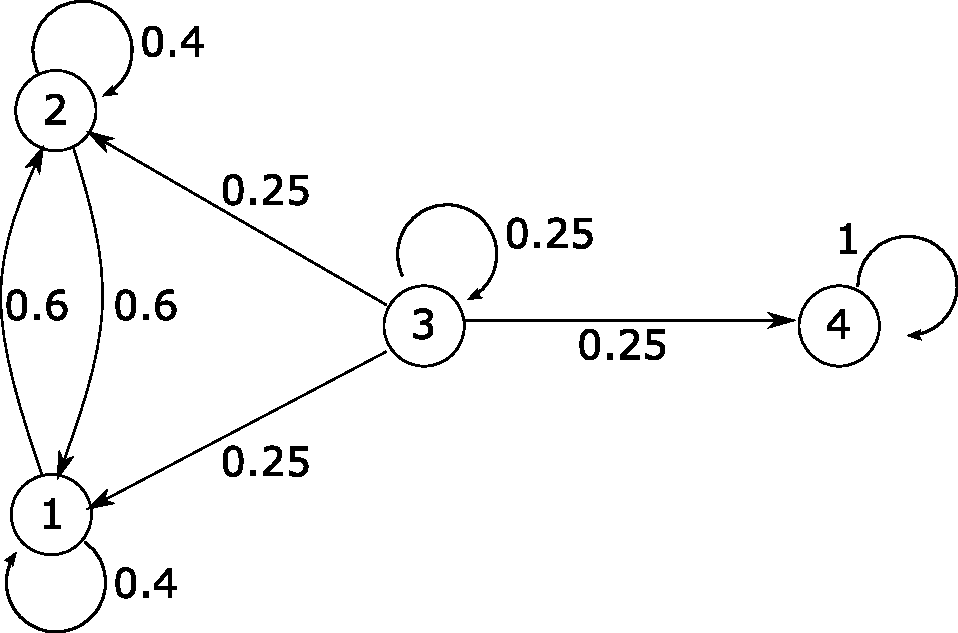
\includegraphics[scale=0.45]{files/Markov.pdf}
        \caption{Four-state Markov Chain \cite{brilliantMarkov}.}
        \label{img:markov}
    \end{figure}
    It is important to note that Markov chains follow the Markov property, which states: \textit{``The probability of future actions are not dependent upon the steps that led up to the present state''} \cite{brilliantMarkov}. Let $S=\{i_1$, $i_2$, $...$, $i_n\}$ be the set of possible states, a Markov Chain can be defined as sequence of random variables $X_1$, $X_2$, $X_3$, $...$ such that
    \begin{equation}
    	\forall n\in \mathbb{Z^+}, \quad P(X_n = i_n \mid X_0 = i_0, \, X_1 = i_1, \, \dots, \, X_{n-1} = i_{n-1}) = P(X_n = i_n \mid X_{n-1} = i_{n-1}),\quad i_k\in S
    \end{equation}

  \subsection{Bayesian Analysis}
    Bayesian Analysis can be defined as a set of practical methods for making inferences from data using probability models for quantities we observe and about which we wish to learn \cite{gelman2013bayesian}. The Bayesian Analysis is another approach to data analysis, just like Frequentist Analysis. Both approaches have their advantages, even though they do not share a similar methodology.
  \subsubsection{Bayesian vs. Frequentist}
  	\textbf{Frequentist}\\ The data to be analyzed is a result from random processes, therefore the data will change each time it is collected. The probability analyzed is
	\begin{equation*}
		P(y\mid\theta)
	\end{equation*}
    where $y$ is the known dataset and $\theta$ are parameters that were used to generate the random dataset. The problem to address by Frequentist Analysis is creating estimators in order to assign values to $\theta$. One big difference between Bayesian and Frequentist is that the second one has to create an estimator for each problem, while the Bayesian only uses one estimator: Bayes Formula.\\
    \textbf{Bayesian}\\ The opposite is considered: data is not random once it has been collected. The parameters, on the other hand, are considered random and a probability distribution is used to model its uncertainty, in other words, to model how much we know about an specific parameter. The probability analyzed is
    \begin{equation*}
    	P(\theta\mid y)
    \end{equation*}
    where $y$ is fixed, $\theta$ is fixed, but the knowledge about it will change. This is often addressed as ``inverse probability'', since you have a set of effects (often is the dataset) and you want to infer the causes. The Bayesian model is useful and flexible, it can be applied to a wide variety of problems; another advantage is that everything is addressed as a probability and, since people often have an intuitive idea of probabilities, the model and the results can be easy to interpret by almost everyone \cite{youtube1}.

  \subsubsection{Steps for a Bayesian Probability Model}
  According to Gelman \cite{gelman2013bayesian}, there are three general steps in order to build a Bayesian model, these are:
    \begin{enumerate}
    \item \textbf{Specify a Probability Model:} Build a model that includes everything that is influential and that you are interested to learn about.
    \item \textbf{Calculate a Posterior Distribution:} The posterior distribution $P(\theta\mid y)$ is referred as posterior because it tells us what we know about the unknown $\theta$ after having observed $y$. It is a function of the probability model we specified in last step. The difficulty in calculating the posterior distribution is the main reason why the adoption of Bayesian Analysis is poor. It is hard to calculate it analytically. But, if you manage to calculate the posterior distribution, you can get:
    \begin{multicols}{2}
    \begin{itemize}
    \item Point estimates
    \item Credible Intervals
    \item Quantiles
    \item Predictions
    \end{itemize}
    \end{multicols}
    \item \textbf{Check your Model:} As everything is represented with the model, is crucial its revision and check. Questions like: does the model fit the data? Are the conclusions reasonable? Are the outputs sensible to changes in the model structure?, can help determine whether the model is working properly or something needs to be rearranged \cite{youtube1}.
    \end{enumerate}

    \subsubsection{Bayes Formula}
    	As it was said before, Bayesian Analysis only uses one estimator: Bayes Formula. This formula was proposed by Thomas Bayes as follows \cite{youtube1}:
        \begin{equation}
        	P(\theta\mid y)=\frac{P(y\mid\theta)P(\theta)}{P(y)}
        \end{equation}
        Where
        \begin{itemize}
        	\item $P(\theta\mid y)$ is the posterior distribution.
            \item $P(\theta)$ is called the Prior, this is what we know about the unknown quantity before observing the data. This is the information state of parameters and it can be used to include information from previous studies, hence, the name Prior.
            \item $P(y\mid\theta)$ is called likelihood distribution. This is the representation of the observed data and it is used to update the prior distribution to posterior distribution. This distribution is closely related to a probability density function. This distribution holds a dataset $y$ constant and looks up which parameter $\theta$ is more likely to have generated that dataset.
            \item $P(y)$ is a normalizing factor, it can be calculated through the law of total probability as follows (depending on the type of data we are working on):
			\begin{equation}
				\begin{split}
               P(y)&=\sum_iP(y\mid\theta_i) P(\theta_i)\\
                    	&=\int P(y\mid\theta)P(\theta)d\theta
				\end{split}
			\end{equation}
        \end{itemize}

\subsubsection{Bayesian Inference in Video Games}
When applying bayesian inference in video games, it is a little different to the formal definition for making it useful in this context. First of all, the data prior to the observation will be the state that the variables that determine the behavior of the player; in this manner, this $y$ is considered as all the values that this variables have at some time $t$. On the other hand, the $\theta$ is represented by the state of another variable at a instant of time forward to the measure before. Likewise, the prior distribution just represents how likely is that the variables we are measuring have some arbitrary state. This is important to highlight, because this method of inference can allows us to infer the position of a object with respect to some measures before, in which state a character is and so forth. Generally, the discrete uniform distribution is used in this types of context due to the fact that most variables in video games take some finite set of values and, are equally likely that the variables takes those values \cite{coue2003using}.

Therefore, this type of inference is different in respect to other applications you might find but still does everything the other ones do.

\section{Contributions \& Application}
As it was discussed in the introduction, Bayesian statistical analysis is very useful in video games to make bots learn certain behavior, specially in complex behavior such as bots in first person shooters, where they have to take into account many variables (it's health, weapon, position in the map, etc.). Therefore, the idea is to apply this concepts and methods in a simpler video game, to see how can it improve the experience playing more directly. Consequently, we chose the video game PacMan to suit this needs.

\subsection{Why Pac-Man?}

PacMan was a video game released in 1979 by Toru Iwatani. Nowadays is considered one of the most influential video games in culture and, was the second game, after Pong, to have such a big visibility reaching to audiences worldwide \cite{pac}. On the other hand, although its massive impact it has had all over the world it does not mean that the game is flawless. As the video game industry was at a very early stage, PacMan's developers lacked algorithms to improve aspects of the game; players have criticized how unresponsive the controls can be, the ghosts don't present much difficulty to the player and more. 

Hence, applying the algorithms of Bayesian Inference in this type of game can illustrate in a very easy manner the benefits of this algorithm. On the other hand, as the game is so simple it allows for the methods to be quite easy, as there are not as much variables as in more complex games. On the other hand, the ghosts in the game are handled using finite state machines (\ref{subsec:finite}) so it has room to be improved upon by this methods. For this reason, we will use this methods to improve the difficulty of the ghosts in the game. The original code in Python can be found in \cite{pac1}.

\subsection{Bayesian Application in Pac-Man}
In this manner, we will use Bayesian inference and Markov chains to make the ghost go to the place that the player will more likely be. The real code, just solves a graph problem by searching for the shortest route to reach where the player is; but, this type of algorithm has problem to difficult the things for the player. On first glance, most of the time you are just being followed by the ghosts and it is very easy to escape them; more often than not, you lose by accident because of the controls are not very good. In second place, all the ghosts, have a very similar behavior due to that they tend to coincide in similar places.


It is important to highlight that PacMan's map is handled as nodes that are every edge in which the player can change it's direction; so, what the ghosts will do is search what is the most likely node that the player is going to go next given its coordinates in the map and its velocity. This is where the uncertainty comes from since, knowing this data allows us to know where exactly is the player going to go in the next time; in this order, thats why we consider at what node will he go at some time plus a random constant. On the other hand, as we are considering nodes and not coordinates  it has another level of uncertainty.

Therefore, we'll have the next variables to make our model:

\begin{table}[H]
\centering

\begin{tabular}{l p{8cm}}
\hline
 $N_{t+k}$ & This is the node that the player is going to be in the time $t+k$.  We don't consider the node in $t+1$ because, as it was expressed earlier, this is deterministic. This will be the variables we'll be interested in to decide the trajectory of the ghost.\\
 $P_t$ &  This is a pair of coordinates $(x,y)$ of the place where the pacman is at time $t$.\\
 $V_t$ &  This is a vector of velocities $(velX,velY)$ that represents the velocity that the pacman has at time $t$. It is important to acknowledge that the velocity at every time has only one dimension, due to that the player can not move diagonally.\\ \hline
\end{tabular}
\caption{Model variables.}
\end{table}



Hence, it is obvious that the behavior that the ghost is going to have is represented by a Markov Chain, with the probabilities calculated respect to the position on the player.

Consequently, the behavior will, when the level begins, each ghost will move randomly to a node so each ghost has a different time to reach the player. On the second hand, when each ghost reaches that random node they will calculate what is the most probable node in which the pacman will go next and, find the shortest path to that node; it's important to notice that if we calculated this node very time the player moves, the game would be impossible to play as every move will be very slow. Therefore, to solve this problem, the ghost will choose a path to the most probable node and follow that even if the player changes it's direction; finally, when they reach the end of the path, they will do the same process and so forth.

In particular, we will need to calculate the probability with Bayes theorem, which in our case is:

\begin{equation}
P({ N }_{ t+k }=n\mid { P }_{ t }=p\wedge { V }_{ t}=v)=\frac{P({ P }_{ t }=p\wedge { V }_{ t}=v\mid{ N }_{ t+k }=n)P({ N }_{ t+k }=n)}{P({ P }_{ t }=p\wedge { V }_{ t}=v)}
\end{equation}

The important tasks to make this model work to calculate accurately this probability is, in first place, to find the model for the posterior distribution. This requires to find the joint distribution of both random variables $P_t$ and $V_t$ that we'll consider both are independent of each others, making it easier to calculate the probability of the random vector of this two variables. On the other hand, it is indispensable to find the likelihood distribution. Lastly, it is necessary to find a probability model that represents the prior.
\section{Results}
\subsection{Modeling Bayes Formula}
\subsubsection{Choosing the Time Limit of Predictions}
On first glance, the most important thing to calculate was the $k$ value, which represented at what time in the future we need to see what is the most probable node that the player is. This value is very important to calculate due to the fact that this constant limits the amount of distance that the PacMan can travel. For convenience issue, we chose this value in the interval $1 \le k \le r$, with $r$ the minimum amount of moves that the ghost needs to reach the player in his actual position. It is important to highlight, that for bigger values of $r$ the prediction is going to be better but, it costs efficiency to the algorithm; on the other hand, this value does not have any limit as, theoretically speaking, the player could go right and left infinite times staying in the same place.

So, the considerations made for this value are to prioritize efficiency at running the algorithm and, this value allows to have a good guess about the optimal move.

\subsubsection{Modeling the Likelihood Distribution}
Now that $k$ has some boundaries, it is important to find all the distributions to calculate this probability. To make this, the game was played by 6 people and recollected data of given a arbitrary position how many times did he move without backtracking. For instance, we count how many moves he made to that place without backtracking; so, if he moved to the right $k-1$ times and to the left the move that was remaining, we considered as a $k-1$ move and so forth. We recollected data from 87 moves with $k$ fixed to the value of 5 and the data recollected can be found in Figure \ref{img:data}.

	  \begin{figure}[H]
          \centering
          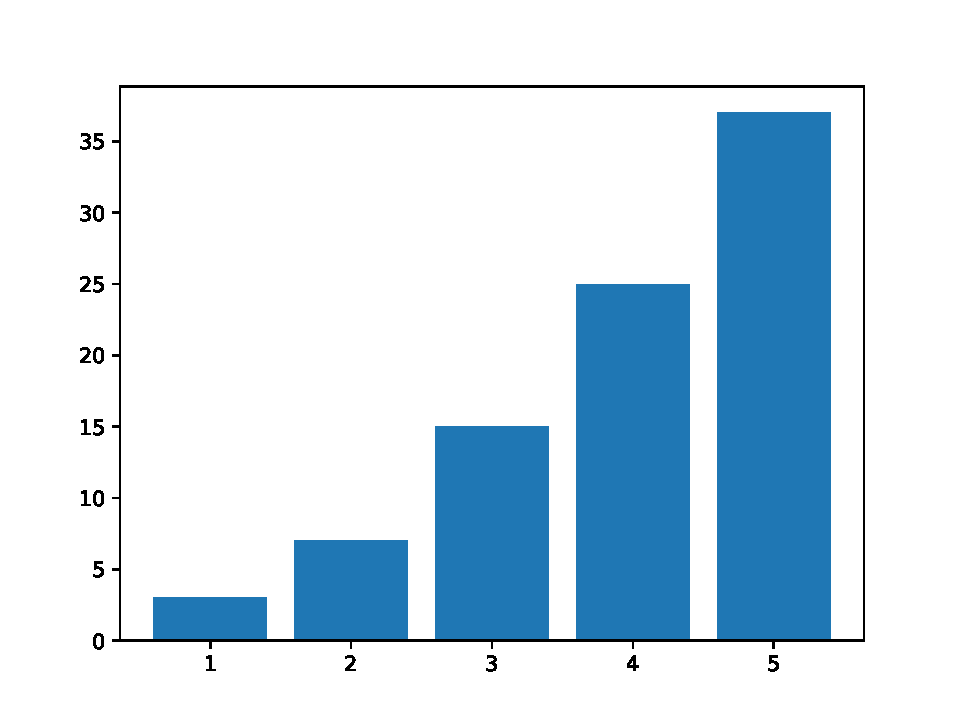
\includegraphics[scale=0.5]{files/Figure_1.pdf}
          \caption{Data recollected of moves of pacman.}
          \label{img:data}
      \end{figure}
      
In this manner, we found that more often than not the player does not back track the move he already made. This is due to the fact that, generally, the player is trying to advance to finish the level by eating all of the points in the map; at the same time, they backtracked only where they were surrounded by ghosts or, they are in vulnerable mode, which leads to take uncommon routes just to kill the enemies.

In conclusion of all of the above, we found that the probability is proportional to the number of movements that the player makes without backtracking to reach that place. Hence, this can be associated to the model of the probability in which node is the player in given a point where this is. Therefore, with this finding we obtain our probability density model for the ${ P }_{ t }=p\wedge { V }_{ t}=v\mid{ N }_{ t+k }$, which is (with $b$ as the number of backtracks the player makes to get to that node respect to the position p):
	\begin{equation*}
      P({ P }_{ t }=p\wedge { V }_{ t}=v\mid{ N }_{ t+k }=n) \quad \alpha \quad (k - b)^2
  \end{equation*}
  \begin{equation*}
      P({ P }_{ t }=p\wedge { V }_{ t}=v\mid{ N }_{ t+k }=n) = \frac {(k - b)^2}{C}
  \end{equation*}

It is important to stand out that $k$ can be calculated as the Manhattan distance from the ghost to the player. Finding $C$ such that this is a probability function, we conclude that the model of the prior distribution is given by:

\begin{equation}
	P({ P }_{ t }=p\wedge { V }_{ t}=v\mid{ N }_{ t+k }=n) = \frac{6(k-b)^2}{k(2k^2 + 3k +1)}, \quad 0 \le b \le k-1
\end{equation}

This equation found is very convenient, although it doesn't represent fully the graph we found in figure 3. On the other hand, we don't need full precision to calculate this probability as, in the long run, we only need to compare which is bigger to decide the movement of the ghost; on the other hand, it would be more appropriate to suppose that this probability is proportional to a power of $k$ for more precision and move the value of the power till finding the exact graph but, we leave it as a suggestion for future work. In this manner, we find that the model found (see the model's graph in Figure \ref{img:real}) is a good approximation of the real model and, it's useful enough for the purpose that it has. 

On the other hand, it is important to emphasize that the likelihood distribution also depends of the velocity of the player but, our model doesn't include this variable. In this manner, we couldn't find a direct correlation between the velocity that the player has and it's relationship to the node; at the same time, this variable is fundamental for calculating later probabilities and for the model to work. 
	\begin{figure}[H]
          \centering
          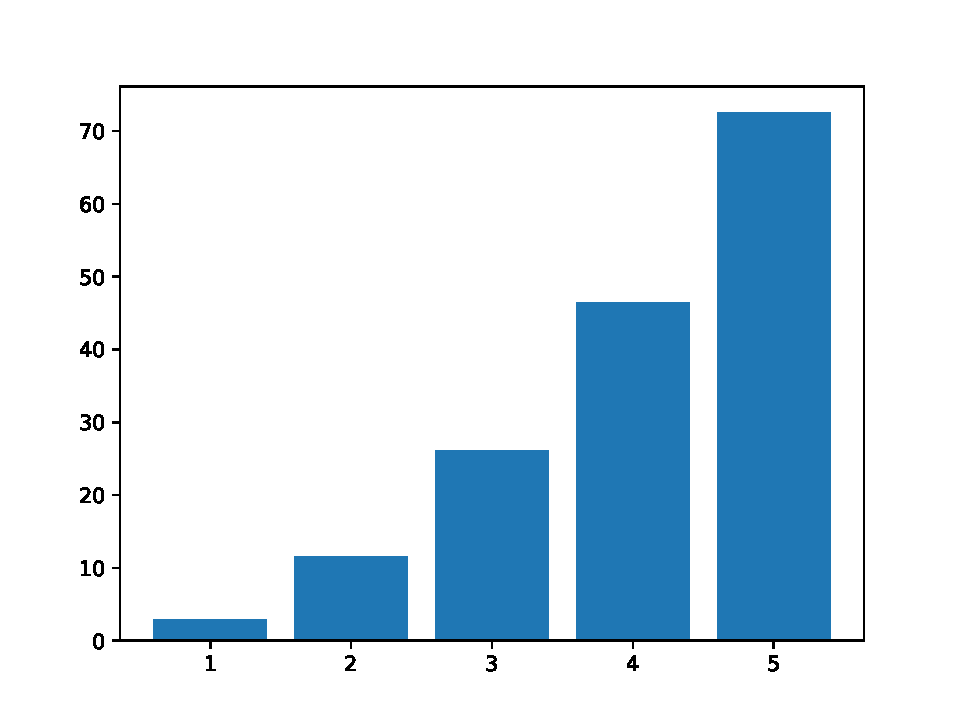
\includegraphics[scale=0.5]{files/Modelo_Teorico.pdf}
          \caption{The same data simulated know by the model found in equation 9.}
          \label{img:real}
      \end{figure}
      
To conclude, it's important to mention that for finding this model it required a lot of peaking and tweaking for making it match the data. In this manner, Bayesian Analysis is a great tool specially for modeling markov chains behavior in video game characters; but, it is difficult to build models to improve the difficulty of the enemies. For future work, we suggest developing tables as seen in the reference \cite{coue2003using} for handling behavior in a easier manner.


\subsubsection{Modeling the Normalizing Term}
As it has already been said, the events of the enemy being in a point $P_t=p$ at a time $t$ and it having a velocity $V_t=v$ are going to be considered as independent events. Therefore, as it was shown in the theory (\ref{subsec:joint}), this normalizing term will be
\begin{equation*}
	P(P_t=p\wedge V_t=v)\,=\,P(P_t=p)P(V_t=v).
\end{equation*}
 Both of the distributions for $P_t$ and $V_t$ will be considered as uniform, since the number of points in the game panel is constant, though it depends on the size of it (which varies depending on the level); on the other hand, there are only 4 possible velocity vectors on each point $p$ at every time $t$, and there is not preference on any of this vectors.
 
Let us define $h$ as the height of the game panel, and $w$ its width; therefore, the uniform density for the random variable $P_t$ will be
\begin{equation}
	P\left( P_{t}=p \right)=
    \begin{cases}
    \frac{1}{wh} & [[0,w]]\times[[0,h]] \\ 
    0 & \text{any other case}
    \end{cases}
\end{equation}
Note that a point $p$ is given by a $(x,y)$ coordinate, and [[a,b]] represents the \textbf{discrete} interval from $a$ to $b$, this is $[[a,b]]=\{a,\,a+1,\,a+2,...,\,b-1,\,b\}$ with $a,\,b\in\mathbb{Z}$. It can be proved that this is, effectively, a density function.

On the other hand, the density function for the velocity vectors will be
\begin{equation}
	P\left( V_{t}=v \right)=
    \begin{cases}
    \frac{1}{4} &  v\in\{(velX,0),(0,velY),(0,-velY),(-velX,0)\}\\ 
    0 & \text{any other case}
    \end{cases}
\end{equation}
As it was discussed in the contributions, the vector can only have one component at a time $t$; it is obvious that this is a density function.

\subsubsection{Modeling the Prior Distribution}
Just as the normalizing factor's marginal distributions, the prior distribution $P(N_{t+k}=n)$ will be a uniformly distributed, since the probability of the player being in any node at a time $t+k$ is the same for all nodes, there will not be preferences for any areas in the game layout. Hence, the density function for $P(N_{t+k}=n)$ is

\begin{equation}
	P\left( N_{t+k}=n \right)=
    \begin{cases}
    \frac{1}{M} &  n\in[[0,M]]\\ 
    0 & \text{any other case}
    \end{cases}
\end{equation}
Where $M$ is total amount of nodes in the games' layout.

Taking all of the above, we end with a posterior distribution:

\begin{equation}
P({ N }_{ t+k }=n\mid { P }_{ t }=p\wedge { V }_{ t}=v)=\frac{24wh(k-b)^2}{Mk(2k^2 + 3k-1)}
\end{equation}

\subsection{Results: Bayesian Inference vs Graph Method}
The algorithm for applying this formula is straightforward. First, as the level starts it sets all the parameters that the distribution needs to calculate the probability; on second place, we set a random node to every ghost so each of them has a different distance from the player; on third place, when the ghost reaches that random node it calculates it's distance to the player and runs an algorithm that finds all of the nodes at a Manhattan distance \cite{manhattan} less tan $k$; finally, it searches for the node with the biggest probability that the player is going to be, and finally moves there.

Although the opposite was thought, the game ran smoothly, even computing bayesian inference constantly. For our tests, the game was played 20 times with the old algorithm (graphs) and the time until the first loss was reported; on the other hand, it was played 40 times after having deployed the new approach (bayesian inference) and, as well, the time until the first defeat was reported. Note that the game with bayesian inference was played slightly more times since it was important to corroborate the proper performance of the ghosts in game and prove that, indeed, they can defeat the player more easily.

This time results are summarized in Table \ref{tab:timeresults}, using common mean calculation, the maximum and the minimum of the data collected; and the complete data for both before and after the model proposed was deployed, is shown in Figure \ref{img:timeresults}.
\begin{table}[H]
\centering
\caption{Game time results before and after the algorithm was deployed.}
\label{tab:timeresults}
\begin{tabular}{ccc}
\hline
\textbf{Quantity} & \textbf{Graph Approach} & \textbf{Bayesian Approach} \\ \hline
\textbf{Mean}     & 24.77                   & 14.75                      \\
\textbf{Max}      & 28.01                   & 20.09                      \\
\textbf{Min}      & 23.56                   & 14.75                     \\ \hline
\end{tabular}
\end{table}
\begin{figure}[H]
  \centering
  \begin{subfigure}[H]{0.4\textwidth}
    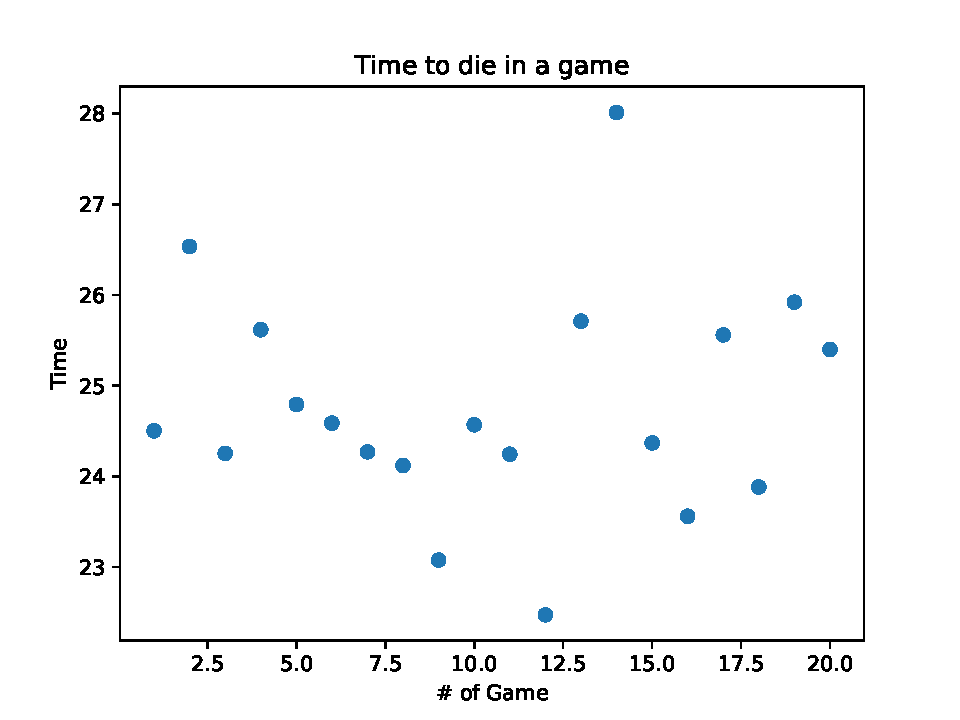
\includegraphics[scale = 0.5]{files/CodigoViejo.pdf}
    \centering
    \caption{Results using graph approach.}
  \end{subfigure}
  \hspace{1cm}
  \begin{subfigure}[H]{0.4\textwidth}
    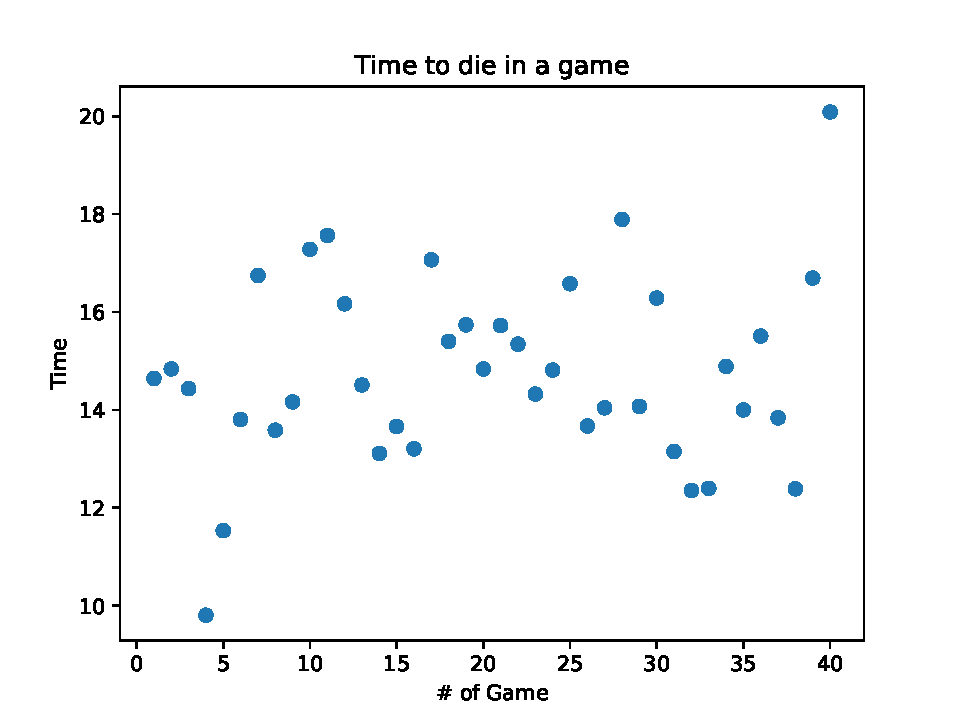
\includegraphics[scale = 0.5]{files/CodigoNuevo.pdf}
    \centering
    \caption{Results using bayesian approach.}
  \end{subfigure}
  \caption{Time until defeat in PacMan.}
  \label{img:timeresults}
\end{figure}

As it is shown in the previous figures, we can affirm that the algorithm is achieving its goals: making a slightly harder gameplay, trying to predict where the player will be and making the overall experience more challenging.













\section{Conclusions \& Future Work}
\subsection{Conclusions}
The application of the algorithm and all of the mathematical modeling was successful to achieve the initial objective of making the ghosts more difficult, in comparison to the normal algorithm. The ghost behavior using Markov Chains instead of the commonly used Finite State Machines is more effective and, at the same time, more useful for teaching different behaviors to enemies.

In second place, we found how this types of algorithm using Bayesian Analysis can help to model behavior in an easier way. In this manner, this paper shows that to teach characters to behave a certain way it is only necessary to find probabilities that determine its response. Using the same method, we could model more difficult behaviors in different games, just mentioning distributions that help write its movement. To look in a more complex example, look in \cite{coue2003using}.

Lastly, even though there was achieved a good result that changes drastically the movement of the ghosts, it still has some errors that could not be accomplished in this paper. For example, many times ghost act very similarly to each other, making it a very unpleasant as it seems too much robotic and not as natural as the game needs to feel. 

\subsection{Future Work}
Knowing that some assumptions were made for modeling the enemies' movement in PacMan, we could consider building non-parametric statistical models for a more appropriate representations. For instance, assuming that the random variables involved in the normalizing term are independent or assuming the uniform distribution of some variables could have led to not optimal results. Another possible aspect to be considered in future work could be including more variables that affect the inference model, for instance, score, level, time, etc. Lastly, for a future research, the usage of a slightly more complex video game could be considered, and like this, scaling the methodology into modern games.


\nocite{*}
\bibliographystyle{ieeetran}
\bibliography{ref}


\end{document}
